\documentclass[a4paper, 11pt]{article}
\usepackage{geometry}
\usepackage{amsfonts, epsfig}
\usepackage{amsmath}
\usepackage{wrapfig} % for wrapping text around figures and tables
\usepackage{graphicx}
\usepackage{float}
\usepackage{multirow}
\usepackage{fancyhdr}
\usepackage{booktabs} % for better table rules
\usepackage{caption} % to customize caption format
\usepackage{linegoal} % for determining the remaining width of the line
\usepackage[backend=biber, sorting=none]{biblatex}
\usepackage{subcaption}

% reference file
\addbibresource{AI.bib}

% \geometry{
%     left=20mm,
%     right=20mm,
%     top=20mm,
%     bottom=20mm
% }

% header and footer
% \makeatletter
% \pagestyle{fancy}
% \def\@oddhead{\parbox{\textwidth}{\raggedright\sffamily\underline{Question 1 - Visualization and analysis of the Palmer penguin dataset} \hfill \thepage}}
% \pagestyle{empty}
% \makeatother

% Define custom page style
\fancypagestyle{nofooter}{
  \fancyhf{}
  \fancyhead[L]{Student Number: 2489941}
  \fancyhead[C]{Introduction to AI}
  \fancyhead[R]{\thepage}% 
  \renewcommand{\headrulewidth}{0.4pt}% Header rule
}
% Apply custom page style
\pagestyle{nofooter}


% Redefine the table and figure formats to bold
\captionsetup[table]{labelfont=bf}
%\captionsetup[table]{labelfont=bf, justification=centering,skip=-2pt}
% \captionsetup[figure]{labelfont=bf}
\captionsetup[figure]{labelfont=bf, justification=centering}
\captionsetup{font=small}

\begin{document}

\begin{center}
  \subsection*{Q1 - Visualization and analysis of the Palmer penguin dataset}
\end{center}

\noindent
The Palmer penguin dataset consists of 344 records of the physical attributes of three species of penguin 
living on three islands in Antarctica (Table~\ref{tab:dataset}) \cite{PM}. 
\begin{wraptable}{r}{0.7\textwidth} % {alignment}{width}
  \small
  \begin{center}
  \vspace{-1.7\baselineskip} % Remove space before the table
  \setlength{\abovecaptionskip}{5pt}
  \setlength{\belowcaptionskip}{5pt}
  \fontsize{10}{10}\selectfont % Change font size here
  \begin{tabular}{l|l|l|l}
  % \begin{tabular}{|p{1.8cm}|p{1.2cm}|p{4cm}|p{1.8cm}|}
  \textbf{Feature}&\textbf{Type}&\textbf{Values in the dataset}&\textbf{Importance}\\
  \hline
  island&categorial&Torgersen, Biscoe, Dream&\ \ \ 0.12 (4)\\
  bill length&numerical&32.1mm - 59.6mm&\ \ \ 0.37 (1)\\
  bill depth&numerical&13.1mm - 21.5mm&\ \ \ 0.17 (3)\\
  flipper length&numerical&172mm - 231mm&\ \ \ 0.23 (2)\\
  body mass&numerical&2700g - 6300g&\ \ \ 0.11 (5)\\
  sex&categorial&Male, Female&\ \ \ 0.01 (6)\\
  species&categorial&Adelie, Chinstrap, Gentoo&\ \ \ \ class\\
  \end{tabular}
  \vspace{-2\baselineskip} % Remove space before title
  \end{center} 
  \caption{\centering\linespread{0.8}\selectfont Palmer penguin dataset features. Importance was calculated using random forest and a ranking is shown.}
  \vspace{-1\baselineskip} % Remove space after the table
  \label{tab:dataset}
\end{wraptable}
In this report, consideration is given to data cleaning and preparation, 
the dataset is then explored through visualization and analysis is carried out 
to compare the accuracy of a small number of AI approaches in classifying penguin species.


\vspace{\baselineskip}
\subsection*{Data cleaning - missing values, encoding, standardization and imbalance}

\begin{wrapfigure}{r}{0.5\textwidth} % {alignment}{width}
  \centering
  \vspace{-1.2\baselineskip} % Remove space before the table
  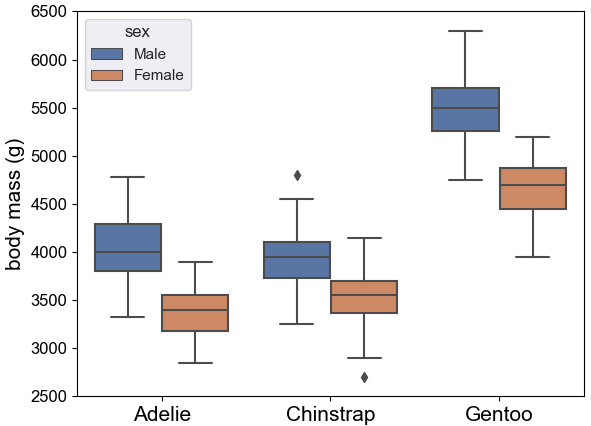
\includegraphics[width=0.48\textwidth]{sex.png} % Adjust the width as needed
  \vspace{-0.5\baselineskip} % Remove space before title
  \caption{\centering\linespread{0.8}\selectfont All numerical features show a significant statistical difference between male and female, 
  as in the body mass example above. Shown are median values, upper and lower quartiles, 
  and outliers.}
  \vspace{-0.5\baselineskip} % Remove space before title
  \label{fig:sex}
\end{wrapfigure}   

The two records missing the sex amd all numerical features were removed as imputation is unlikely to be reliable. 
The remaining nine records are missing only the sex attribute. Figure~\ref{fig:sex} shows the physical 
attributes of the male and female of each species differ statistically and so it is reasonable to 
consider imputing sex for those records. Following standardization, 
a Shapiro-Wilk test confirmed each numerical attribute has a normal distribution \cite{shapiro1965analysis} 
and separate Z-tests were applied to assess the 
hypotheses that the missing sex value is male or female \cite{freedman2007statistics}. 
Two of the records could be imputed as male and three as female 
and these were retained, with the remaining four records being removed. 
The cleaned dataset has 338 records, 147 Adelie  
(74 male, 73 female), 68 Chinstrap (34 male, 34 female) and 123 Gentoo (62 male, 61 female).

The categorical features in the dataset were encoded to numerical values. `One-shot' encoding of 
categorical features was considered but not found to 
improve performance. A number of AI methods are known to be biased in favour of numerical features 
with smaller standard deviations \cite{hastie2009elements}, but this can be reduced by standardization 
of features to zero mean and unity standard deviation. In this work, 
standardization statistics were calculated only from training sets, but applied to all data. 
If a dataset is imbalanced, 
AI predictions may be biased towards classes more frequently found in the training data. 
In the Palmer penguin dataset, the number of Chinstrap records is around half of that for either Adelie or Gentoo, 
but, as all the methods adopted in the current work are known to be little affected by 
imbalanced data \cite{he2009learning}, no modifications were made.

% \vspace{\baselineskip}
\subsection*{Visualization of the dataset}

\begin{wrapfigure}{r}{0.53\textwidth} % {alignment}{width}
  \centering
  \vspace{0\baselineskip} % Remove space before the table
  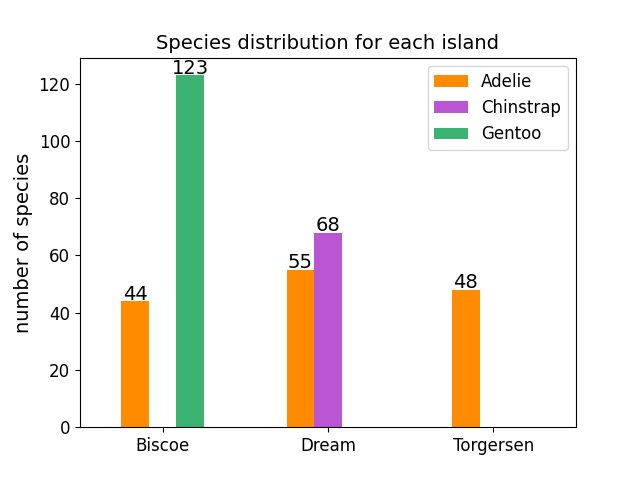
\includegraphics[width=0.48\textwidth]{islands.png} % Adjust the width as needed
  \vspace{-0.5\baselineskip} % Remove space before title
  \caption{\centering\linespread{0.8}\selectfont Adelie is on all three islands, but Gentoo and Chinstrap samples are from only one.}
  \vspace{-0.5\baselineskip} % Remove space after title
  \label{fig:islands}
\end{wrapfigure}
Figure~\ref{fig:islands} shows the species distribution for the islands. 
Chinstrap and Gentoo penguins are found only on one island, making island a potential confounding factor whose 
individual environmental factors may influence physical characteristics. 
A Shapiro-Wilk test confirmed the normal distribution of the numerical features of the Adelie penguins (found on 
all islands) and an ANOVA test confirmed the features are not significantly influenced by the island inhabited. 
It is clear the island is not a confounding factor in the dataset.

\begin{wrapfigure}{r}{0.58\textwidth} % {alignment}{width}
  \centering
  \vspace{0\baselineskip} % Remove space before the figure
  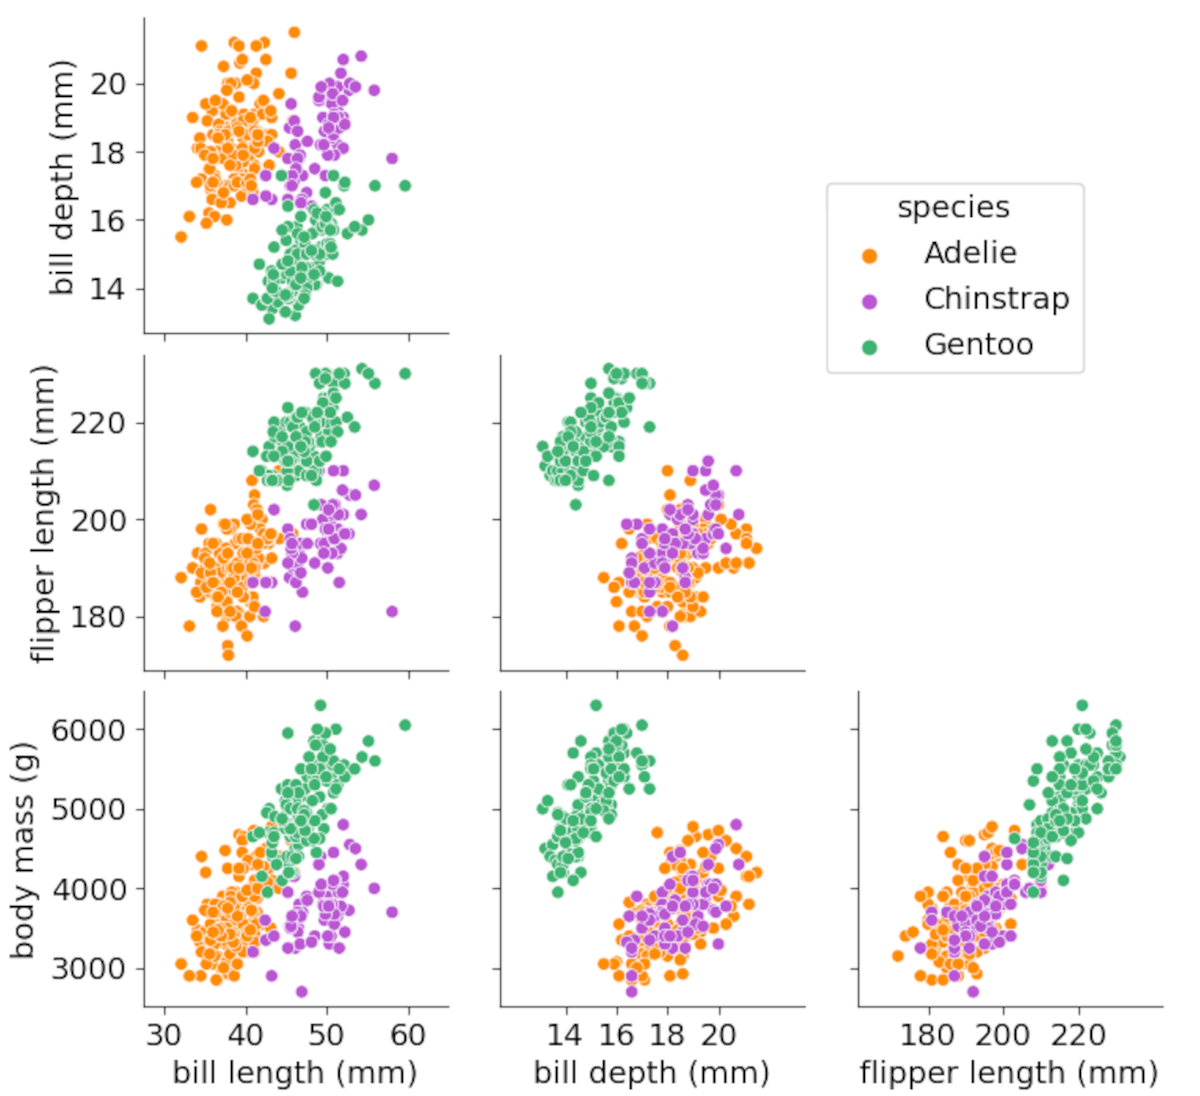
\includegraphics[width=0.58\textwidth]{pairwise.png} % Adjust the width as needed
  \vspace{-1.5\baselineskip} % Remove space before title
  \caption{\centering\linespread{0.8}\selectfont Pairwise distributions of numerical features. Gentoo can be distinguished, 
  but Adelie and Chinstrap may not be completely separable from one another}
  \vspace{-1\baselineskip} % Remove space after title
  \label{fig:pairwise}
\end{wrapfigure}
Table~\ref{tab:dataset} shows the feature importance scores (and rank in parentheses) indicating
relative contributions to predicting the penguin species.
Results reported later show that performance improvements can be achieved by
concentrating classification on the more `important' features.

Pairwise scatterplots for the numerical features are shown in Figure~\ref{fig:pairwise}. 
Bill depth, combined with either flipper length or body mass, 
yields a separable cluster of Gentoo penguins (shown in 
green) allowing them to be identified. 
No pairwise combination completely separates Adelie (orange) from Chinstrap (purple) clusters, 
but the best candidate feature for doing so is in distributions involving bill length.

Figure~\ref{fig:sex} above shows there is a difference in the body masses of the male and female samples for each of the three species. 
Differences between the sexes for the other three numerical physical characteristics in the dataset were also apparent. 
Since narrower distributions are seen if the sex of the species is considered rather than just the species itself, 
including sex is likely to provide a finer grained distinction for species classification 
and this knowledge can be used to improve performance, as discussed in the `results and analysis' section below. 

\subsection*{Methodology}

\begin{wraptable}{r}{0.6\textwidth} % {alignment}{width}
  \small
  \begin{center}
  \vspace{-2\baselineskip} % Remove space before the table
  \setlength{\abovecaptionskip}{5pt}
  \setlength{\belowcaptionskip}{5pt}
  \fontsize{10}{10}\selectfont % Change font size here
  \begin{tabular}{l|l|l}
  \textbf{Method} & \textbf{Metaparameters} & \textbf{Values considered}\\
  \hline
  \multirow{3}{*}{\textit{k}nn}    & nearest neighbours \textit{k}	  & \textit{\textbf{1}}, 2, 3, 4, 5, 6, 8, 10\\
                                   & prediction function	& \textit{\textbf{uniform}},distance \\
                                   & distance metric 	& \textit{\textbf{Manhattan}},Euclid \\
  \hline
  \multirow{6}{*}[0.5ex]{\begin{tabular}[t]{@{}l@{}}random \\ forest\end{tabular}} 
                                   & number of trees & 5, \textit{\textbf{10}}, 15, 20, 25 \\
                                   & maximum depth & \textit{\textbf{no max}}, 10, 20 \\
                                   & min samples to split  & \textit{\textbf{2}}, 5, 10 \\
                                   & min samples at leaf & \textit{\textbf{1}}, 2, 4 \\
                                   & split function & \textit{\textbf{gini}},entropy \\

  \hline
  \multirow{4}{*}{\textit{k}-means} & number of clusters \textit{k}  & 2, \textit{\textbf{3}}, 4, 5, 6, 7, 8, 10\\
                                    & centroid initialize         & \textit{\textbf{k-means++}},random\\
                                    & runs for centroid	     & 2, \textit{\textbf{5}}, 10, 20 \\
                                    & maximum iterations           & 5, \textit{\textbf{10}}, 20, 50 \\
  \hline
    \multirow{3}{*}{CVA}            & regularization   & 0.1, 1, \textit{\textbf{10}}, 100 \\
                                    & kernel coefficient      & \textit{\textbf{1}}, 0.1, 0.01, 0.001 \\
                                    & kernel type                  & rbf, \textit{\textbf{linear}},poly \\
  \hline
  \end{tabular}
  \vspace{-2\baselineskip} % Remove space before title
  \end{center} 
  \caption{\centering\linespread{0.8}\selectfont Metaparameters values shown in italics most consistently produced training results of 
  best accuracy during validation and were selected for generating results}
  \vspace{-1\baselineskip} % Remove space after the table
  \label{tab:metaparameters}
\end{wraptable} 


The code is available on Gitub \cite{TimAIRepo} and was written in Python 3.11 \cite{python311} 
using ‘Scikit-Learn’ libraries \cite{scikit-learn}.
Predicting the penguin species from the given features is a classification problem. 
Results are obtained from two conventional classification approaches, 
namely \textit{k}-Nearest Neighbour (\textit{k}nn) \cite{bishop2006pattern} and random forest \cite{breiman2001random}, 
unsupervised \textit{k}-means (following cluster labelling) \cite{tan2005introduction} 
and a novel combined visualization and analysis (CVA) approach that is a mix of 
practical visualizations and Support Vector Machine (SVM) classification.

\begin{wraptable}{r}{0.58\textwidth} % {alignment}{width}
  \small
  \begin{center}
  \vspace{0\baselineskip} % Remove space before the table
  \setlength{\abovecaptionskip}{5pt}
  \setlength{\belowcaptionskip}{5pt}
  \fontsize{10}{10}\selectfont % Change font size here
  \begin{tabular}{l|l}
  \textbf{Method} & \textbf{Accuracy (range)}\\
  \hline
  baseline, Adeleie species & 43.49\% \\
  \hline
  \textit{k}NN, all features & 99.24\% (97.06\%-100\%)\\
  \textit{k}NN, no island &	99.46\% (97.06\%-100\%)\\
  \hline
  random forest, all features	& 98.57\% (95.59\%-100\%)\\
  random forest, no body mass & 98.49\% (92.65\%-100\%)\\
  \hline
  \textit{k}-means, numerical features & 97.03\% (94.12\%-97.06\%)\\
  \textit{k}-means, two sex clusters  & 99.18\% (94.12\%-100\%)\\
  \hline
  CVA, three main features & 98.98\% (95.35\%-100\%)\\
  CVA, separate sex models & 99.25\% (90.91\%-100\%)\\
  \hline
  \end{tabular}
  \vspace{-2\baselineskip} % Remove space before title
  \end{center} 
  \caption{\centering\linespread{0.8}\selectfont Classification accuracy mean value and range for 100 pseudo-random test sets 
  and using the metaparameters identified in Table~\ref{tab:metaparameters}}
  \vspace{-0.5\baselineskip} % Remove space after the table
  \label{tab:results}
\end{wraptable} 

To reduce the potential for overfitting, the classification methods (all but \textit{k}-means) were trained using 
`holdout validation', where 80\% of the dataset was used in a five-fold cross-validation 
configuration \cite{james2013introduction}. The remaining 20\% was kept for a test set. For all methods, 
the Scikit-Learn function GridSearchCV was employed to tune metaparameters \cite{scikit-learn}. 
Table~\ref{tab:metaparameters} shows the values selected for the metaparameter grid. Those giving the best 
performance were selected to generate accuracy results (the percentage of correctly predicted species) 
from the test set. The metrics `precision' and `recall' were also caculated, but as 
these are only relevant if false positives or false negatives (respectively) are specfically to be avoided, 
they are not included in this report.
\subsection*{Results and analysis}
\noindent
This work used the Scikit-Learn 
pseudo-random procedures for selecting validation and test set values and 100 of these were used 
both when selecting metaparameters and when deriving accuracy results.
The results in Table~\ref{tab:results} include a baseline that is used to demonstrate 
performance improvements achieved by the AI methods considered. In classification, the
baseline method is often simply to select the most frequent class in the observations and, 
in this work, this is the Adelie penguins, giving an accuracy of 43.49\% (147/338).

\textbf{Classification method 1 - \textit{k}nn}  
An additional test was carried to investigate if, compared to the accuracy found for all features, 
the omission of features and combinations of features could improve accuracy.
% \begin{wrapfigure}{r}{0.46\textwidth} % {alignment}{width}
%   \centering
%   \vspace{-0.5\baselineskip} % Remove space before the figure
%   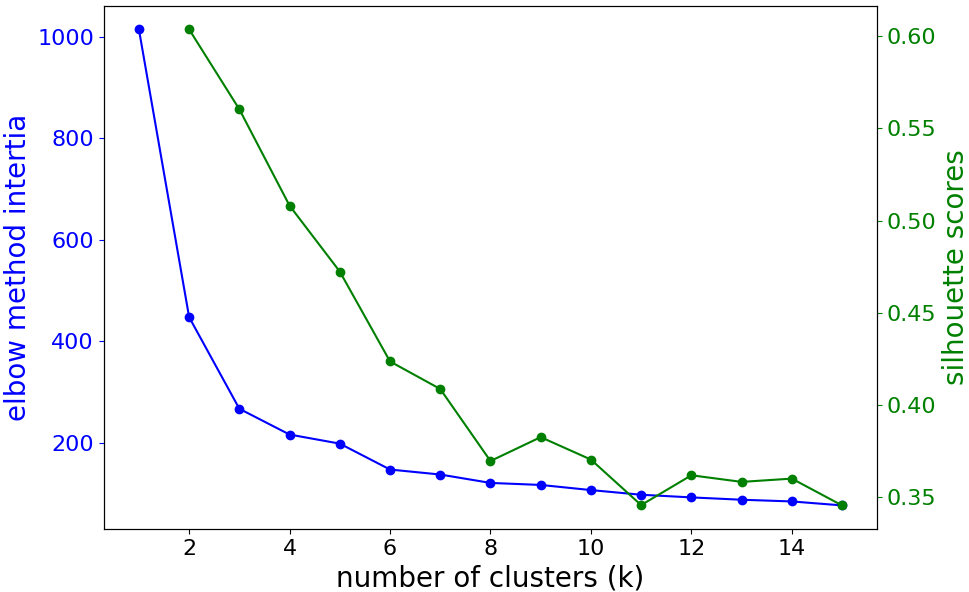
\includegraphics[width=0.48\textwidth]{kmeansvalue.png} % Adjust the width as needed
%   \vspace{-1.5\baselineskip} % Remove space before title
%   \caption{\centering\linespread{0.8}\selectfont The \textit{k}-means elbow is the change in slope of `inertia' (\textit{k}=3)
%   and the silhouette is the `score' closest to 1 (\textit{k}=2)}
%   \vspace{-1\baselineskip} % Remove space after title
%   \label{fig:kmeansvalue}
% \end{wrapfigure}
An improvement was found when island was omitted and when \textit{k}=3. It appears that island did not provide 
any additional information and the higher value of \textit{k} implies better generalization may have been achieved.

\textbf{Classification method 2 - Random forest}  
Including all of the features in the analysis gave an accuracy marginally worse 
than achieved using \textit{k}nn. 
In contrast with \textit{k}nn, no performance improvement was found using fewer features, indicating that random forest
may be less influenced by superfluous features in training data. 
For selected test sets, 100\% accuracy is possible, but the trained systems is likely to exhibit poor generalization.

\textbf{Unsupervised method - \textit{k}-means}  
Although a clustering method, 
\textit{k}-means can be used for classification by matching clusters to classes. 
The \textit{k}-means method is normally applied only to numerical features and only they were included in this work. 
Using the elbow approach, the number of clusters (\textit{k}) was found to 2, but was found to be 3 using the silhouette method.
Empirically, accuracy improved significantly when \(k \geq 4\)
as clusters were not reliably formed for all three species for smaller values of \textit{k},  
Figure~\ref{fig:kmeansmap} illustrates the mapping of classes to clusters for two feature dimensions. 
No accuracy improvement was obtained by reducing the number of features, 
but when a separate set of \textit{k}-means clusters was created for each sex 
this led to a small improvement in accuracy. 

\begin{wrapfigure}{r}{0.5\textwidth} % {alignment}{width}
  \centering
  \vspace{-1\baselineskip} % Remove space before the table
  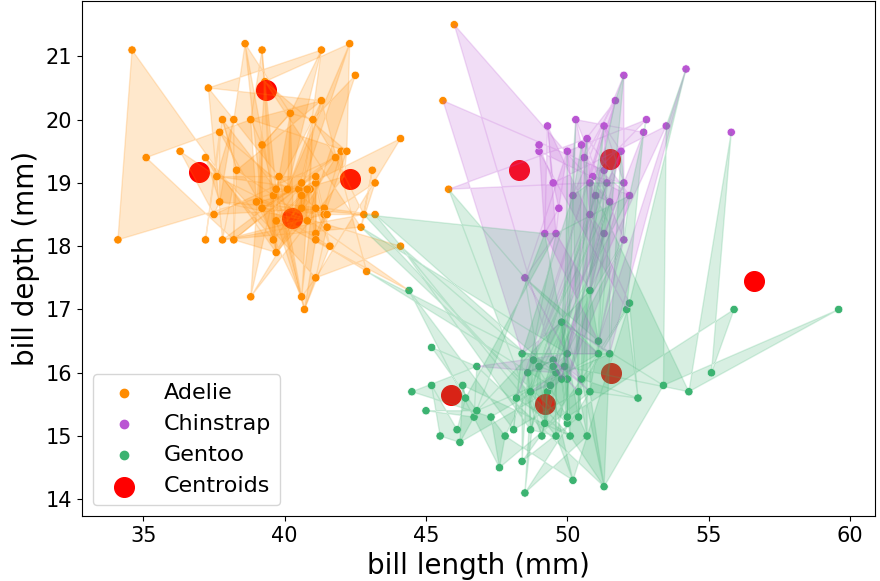
\includegraphics[width=0.48\textwidth]{kmeansmap.png} % Adjust the width as needed
  \vspace{-0.5\baselineskip} % Remove space before title
  \caption{\centering\linespread{0.8}\selectfont \textit{k}-means clusters mapped to species using majority voting. 
  Class assignments are shown by polygon colour (\textit{k}=10, 50 samples coloured).}
  \vspace{-1\baselineskip} % Remove space before title
  \label{fig:kmeansmap}
\end{wrapfigure}

\textbf{A novel combined visualization and analysis (CVA) approach}  
The CVA approach involves visualizing selected pairwise plots of features 
to identify a sequence of two-dimensional SVM classifiers. 

An application of CVA to the Penguin dataset is illustrated in Figure~\ref{fig:CVA}. 
Figure~\ref{fig:CVA}(a) shows the relationship between bill depth and flipper length, and
SVM determines finds a suitable `decision boundary' to separate Gentoo from the other two species. 
Figure~\ref{fig:CVA}(b) plots bill length against bill depth and shows a second SVM line to best separate Adelie and Chinstrap. An improvement in accuracy
was apparent when separate SVM models were developed for each penguin sex.

\begin{figure}[!ht]
    \vspace{-0.5\baselineskip} % Remove space before figure
    \begin{subfigure}{0.47\textwidth}
    \centering
    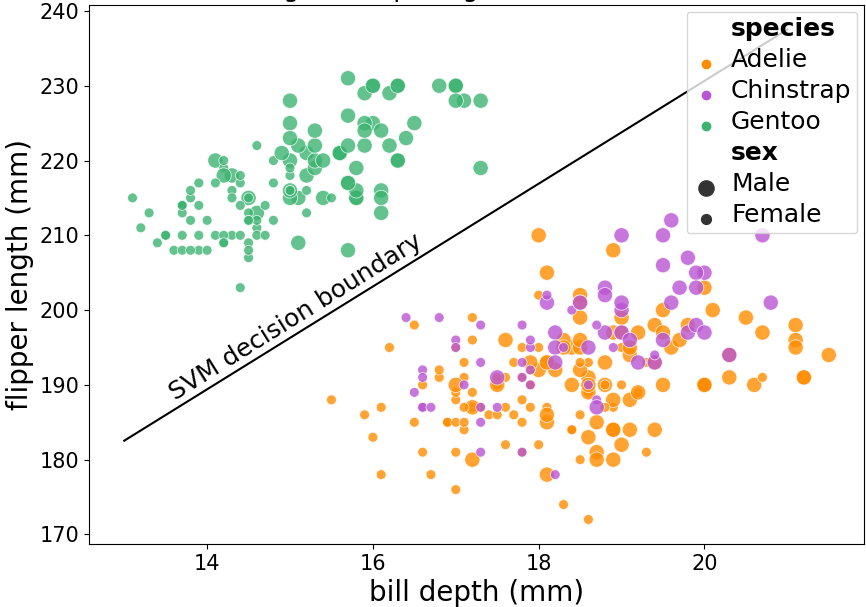
\includegraphics[width=1\textwidth]{sup_fliplen_billdepth.png} % Adjust the width as needed
    \caption{Gentoo can be distingushed from other species}
    \vspace{-1.5\baselineskip} % Remove space before title
    \label{fig:CVA_part_a}
  \end{subfigure}
  \hfill
  \begin{subfigure}{0.47\textwidth}
    \centering
    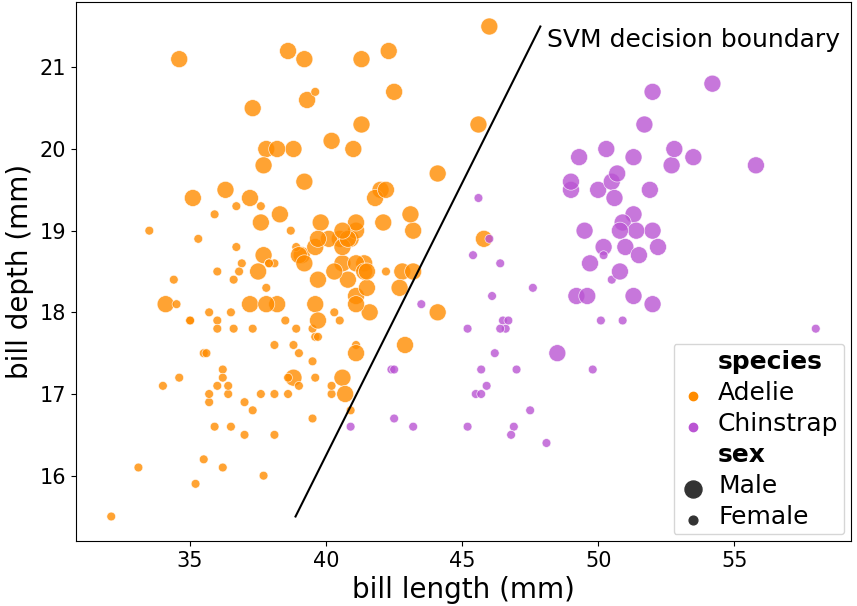
\includegraphics[width=1\textwidth]{sup_billlen_billdepth.png} % Adjust the width as needed
    \caption{Adelie and Chinstrap can be partially separated}
    \vspace{-1.5\baselineskip} % Remove space before title
    \label{fig:CVA_part_b}
  \end{subfigure}
  \vspace{1\baselineskip} % Remove space before title
  \caption{\centering\linespread{0.8}\selectfont Two-stage CVA approach with boundaries fitted using SVM 
  to training data of feature pairs}
  \label{fig:CVA}
  \vspace{-1.4\baselineskip} % Remove space after title
\end{figure}
% \vspace{\baselineskip}
\subsection*{Conclusions}

With careful data preparation, optimization of metaparameters and robust application of training and testing methods, 
the \textit{k}nn and random forest classification methods produced high-quality results. 
As expected, the \textit{k}-means accuracy results were comparitively worse
as in training it does not take advantage of target data information known to the supervised approaches. 

The novel CVA approach was able to produce accuracy results
similar to those of other classification methods. 
Although needing to be tailored to each problem and not well-suited to high-dimensionality data, 
its internal operations are transparent, in contrast with many general-purpose classification methods. 


\begin{center}
\subsection*{Question 2 - Ethical challenges and threats in AI}
\end{center}

\subsection*{Racial Bias in Medical Algorithms}

In 2019, a widely used US healthcare algorithm was found to discriminate by prioritising hospital services based on historical spending records, resulting in the allocation of relatively less future funding and fewer referrals for black patients \cite{Jemielity2019, Ledford2019}. Through the application of a series of test data sets, Obermeyer et al. \cite{Obermeyer2019} identified this inadvertent bias and the team was able to mitigate against it by adjusting the model’s training labels. 

The fact that this third-party assessment and adjustment were possible, demonstrates how exposing a model’s internal operations can aid bias identification and removal \cite{Seroussi2020, Winter2023}. Ensuring greater transparency of AI models is becoming the subject of legislation, for example the 2023 EU AI Act aims to enforce transparency principles by requiring developers to disclose an algorithm’s variables, data sources, and selection logic \cite{EuropeanParliament2023, Edwards2021}. While ensuring that organisations building AI systems are held accountable for the processes used in their development may lead to algorithmic changes that reduce bias \cite{Donovan2018, Lawry2020}, care needs to be taken that the removal of bias doesn't significantly affect the performance of the model in its application domain \cite{Kearns2020}.

\subsection*{AI system safety and existential risks in warfare}

Recent developments in AI have led many researchers to believe that AI systems capable of directly acting in the real world based on decisions they have taken autonomously will become available later this century \cite{Grace2018}. With such advancements comes the risk that AI systems whose decision-making does not prioritise human welfare may pose a threat to life \cite{Ord2020}. 

A specific example of a military AI system posing an existential risk \cite{yampolskiy2016, Cummings2017}, is one that decides maximising human casualties would be the best strategy to achieve a high-level battlefield objective \cite{Barrat2013}. Recent deployments of automated missiles that activate on target acquisition \cite{Atherton2021, BodeWatts2023},  have raised ethical concerns over the use of AI in situations where human beings are potential targets \cite{Emery2021}. If such advanced AI was given control of powerful military weapons and applied more widely, the ramifications for the human race's survival could be profound \cite{Tegmark2017}. 

Addressing these existential threats requires international cooperation to guarantee the transparency of AI algorithms \cite{Cihon2019, Leslie2019}. A potential future safeguard is to include a human-controlled override in all military AI systems \cite{CritchKrueger2020}, although Russell \cite{Russell2019} warns that super-intelligent AI may be capable of removing such safety measures. Ultimately, a global strategy that prioritises human wellbeing in all areas of AI usage will be essential.


\printbibliography


\end{document}
